
\documentclass[aspectratio=169]{beamer}

% activate me to make slides with no animation
%\documentclass[handout]{beamer}


\usepackage[warn]{mathtext}
\usepackage[T2A]{fontenc}
\usepackage[utf8]{inputenc}
\usepackage[english,russian]{babel}

\usepackage{amssymb}
\usepackage{amsmath}
\usepackage{multirow}
\usepackage{graphicx}
\usepackage{verbatim}
\usepackage{comment} 
\usepackage{minted}

\usepackage{listings}
\lstset{language=Java,
                basicstyle=\footnotesize\ttfamily,
                keywordstyle=\footnotesize\color{blue}\ttfamily,
}


%%%%%%%%%%%%%%%%%%%%%%%%%%%%%%%%%  fix-lstlinebgrd.tex 
\makeatletter
\let\old@lstKV@SwitchCases\lstKV@SwitchCases
\def\lstKV@SwitchCases#1#2#3{}
\makeatother
\usepackage{lstlinebgrd}
\makeatletter
\let\lstKV@SwitchCases\old@lstKV@SwitchCases
        
\lst@Key{numbers}{none}{%
    \def\lst@PlaceNumber{\lst@linebgrd}%
    \lstKV@SwitchCases{#1}%
    {none:\\%
     left:\def\lst@PlaceNumber{\llap{\normalfont
                \lst@numberstyle{\thelstnumber}\kern\lst@numbersep}\lst@linebgrd}\\%
     right:\def\lst@PlaceNumber{\rlap{\normalfont
                \kern\linewidth \kern\lst@numbersep
                \lst@numberstyle{\thelstnumber}}\lst@linebgrd}%
    }{\PackageError{Listings}{Numbers #1 unknown}\@ehc}}
\makeatother
%%%%%%%%%%%%%%%%%%%%%%%%%%%%%%%%%


%%%%%%%%%%%%%%%%%%%%%%%%%%%%%%%%%  bListHL
\makeatletter
%%%%%%%%%%%%%%%%%%%%%%%%%%%%%%%%%%%%%%%%%%%%%%%%%%%%%%%%%%%%%%%%%%%%%%%%%%%%%%
%
% \btIfInRange{number}{range list}{TRUE}{FALSE}
%
% Test in int number <number> is element of a (comma separated) list of ranges
% (such as: {1,3-5,7,10-12,14}) and processes <TRUE> or <FALSE> respectively

\newcount\bt@rangea
\newcount\bt@rangeb

\newcommand\btIfInRange[2]{%
    \global\let\bt@inrange\@secondoftwo%
    \edef\bt@rangelist{#2}%
    \foreach \range in \bt@rangelist {%
        \afterassignment\bt@getrangeb%
        \bt@rangea=0\range\relax%
        \pgfmathtruncatemacro\result{ ( #1 >= \bt@rangea) && (#1 <= \bt@rangeb) }%
        \ifnum\result=1\relax%
            \breakforeach%
            \global\let\bt@inrange\@firstoftwo%
        \fi%
    }%
    \bt@inrange%
}
\newcommand\bt@getrangeb{%
    \@ifnextchar\relax%
        {\bt@rangeb=\bt@rangea}%
        {\@getrangeb}%
}
\def\@getrangeb-#1\relax{%
    \ifx\relax#1\relax%
        \bt@rangeb=100000%   \maxdimen is too large for pgfmath
    \else%
        \bt@rangeb=#1\relax%
    \fi%
}
%%%%%%%%%%%%%%%%%%%%%%%%%%%%%%%%%%%%%%%%%%%%%%%%%%%%%%%%%%%%%%%%%%%%%%%%%%%%%%
%
% \btLstHL<overlay spec>{range list}
%
% TODO BUG: \btLstHL commands can not yet be accumulated if more than one overlay spec match.
%
\newcommand<>{\btLstHL}[1]{%
\only#2{\btIfInRange{\value{lstnumber}}{#1}{\color{yellow}\def\lst@linebgrdcmd{\color@block}}{\def\lst@linebgrdcmd####1####2####3{}}}%
}%

\newcommand<>{\btLstHLG}[1]{%
\only#2{\btIfInRange{\value{lstnumber}}{#1}{\color{green}\def\lst@linebgrdcmd{\color@block}}{\def\lst@linebgrdcmd####1####2####3{}}}%
}%
\makeatother
%%%%%%%%%%%%%%%%%%%%%%%%%%%%%%%%%



\usetheme{CambridgeUS}

% tikz
\usepackage{pgf}
\usepackage{tikz}
\usepackage{tikz-qtree}
\usetikzlibrary{arrows, automata, fit, shapes, shapes.multipart, trees, positioning}

\usepackage{array}
\usepackage{cancel}
\usepackage{hyperref}
\usepackage[normalem]{ulem}


\newtheorem{homeworkmail}[theorem]{Homework, mail}

\newcommand{\showTOC}{
    \begin{frame}[noframenumbering,plain]
        \frametitle{Lecture plan}
        \tableofcontents[currentsection]
    \end{frame}
}

\newcommand{\showTOCSub}{
    \begin{frame}[noframenumbering,plain]
        \frametitle{Lecture plan}
        \tableofcontents[currentsubsection]
    \end{frame}
}


\newcommand{\questiontime}[1]{
    \begin{frame}[noframenumbering,plain]
        \frametitle{Question time}

        Question: #1

        \begin{center}
            
\includegraphics[width=0.4\textwidth]{../../common/pics/coins.png}
        \end{center}

        
    \end{frame}
}



\newcommand{\orgNum}{0}
\newcommand{\orgTopic}{org meeting}
\newcommand{\orgKey}{syllabus, contacts}

\newcommand{\introNum}{1}
\newcommand{\introTopic}{introduction to multithreading}
\newcommand{\introKey}{concurrency, parallelism, agents, threads, scheduler, Amdahl's law, race condition, deadlock, wait-for graph}

\newcommand{\basicNum}{2}
\newcommand{\basicTopic}{basic concepts}
\newcommand{\basicKey}{mutex, acquisition order, reentrancy, fairness, data locking, code locking, signalling, condition variable, lost signal, spurious wakeup}

\newcommand{\syncPrimitivesNum}{3}
\newcommand{\syncPrimitivesTopic}{advanced synchronization primitives}
\newcommand{\syncPrimitivesKey}{monitor, latch, barrier, thundering herd, semaphore, read-write lock, thread pool, executor, producer-consumer, fork-join, load balancing}

\newcommand{\patternsNum}{4}
\newcommand{\patternsTopic}{advanced synchronization concepts}
\newcommand{\patternsKey}{interruption, cancellation, partitioning, privatization, replication, thread-local, ownership}

\newcommand{\extraBasicsNum}{5}
\newcommand{\extraBasicsTopic}{additional topics of practical concurrency}
\newcommand{\extraBasicsKey}{documenting protocols and classes, checking concurrent invariants, stress testing, execution trace analysis, estimating required testing effort, static and dynamic checks, scheduling randomization, model checking}

\newcommand{\foundationsNum}{6}
\newcommand{\foundationsTopic}{theoretical foundations of concurrency}
\newcommand{\foundationsKey}{timeline, partial order, sequential consistency, linearizability, quiscent consistency, correctness, liveness, safety, atomicity}

\newcommand{\foundationsPlusNum}{7}
\newcommand{\foundationsPlusTopic}{progress guarantees, concurrent operations hierarchy, consensus number}
\newcommand{\foundationsPlusKey}{obstruction-free, lock-free, wait-free, safe register, regular register, atomic register, consensus number, register snapshots}

\newcommand{\atomicsNum}{8}
\newcommand{\atomicsTopic}{introduction to atomics}
\newcommand{\atomicsKey}{compare-and-swap, fetch-and-add, spinning, lock-free stack, taxonomy of queues, ABA problem}

\newcommand{\cacheCoherencyNum}{9}
\newcommand{\cacheCoherencyTopic}{cache coherency}
\newcommand{\cacheCoherencyKey}{cache memory hierarchy, cache coherency protocol. store-buffer, load-buffer, invalidate-queue, memory barrier, hardware memory model, weak memory model, litmus tests}

\newcommand{\langMMNum}{10}
\newcommand{\langMMTopic}{language memory model}
\newcommand{\langMMKey}{motivation, approaches, comparison of existing solutions}

\newcommand{\advancedConcurrencyNum}{11}
\newcommand{\advancedConcurrencyTopic}{advanced concurrency}
\newcommand{\advancedConcurrencyKey}{CLH/MCS queue/lock, backoff policies revisited, notify-as-ready, RAT optimization, single LIFO cell optimization, work distribution, work stealing, taxonomy of parallel problems}

\newcommand{\userSpaceThreadingNum}{12}
\newcommand{\userSpaceThreadingTopic}{user-space threading}
\newcommand{\userSpaceThreadingKey}{berkley socket, blocking and non-blocking IO, callback-hell, async-await, continuation-passing-style, fibers/coroutines/green threads, stackful vs stackless}


\newcommand{\designNum}{13}
\newcommand{\designTopic}{designing concurrent systems}
\newcommand{\designKey}{park/unpark, synchronizer, futex/wait-on-address, plan9 approach, race-finders, ForkJoinPool/CoroutineCarriers/UIthread, observability, structured concurrency}

\newcommand{\frameworksAndDistributedNum}{14}
\newcommand{\frameworksAndDistributedTopic}{multi-agent systems}
\newcommand{\frameworksAndDistributedKey}{auto-parallelization languages and frameworks, semi-automatic synchronization, distributed systems, consensus protocols}


\title[]{Lecture \basicNum: \basicTopic}
\subtitle[]{\basicKey}
\author[]{Alexander Filatov\\ filatovaur@gmail.com}

\date{}


\newcommand{\taskAsyncException}{2.1}
\newcommand{\taskEmpire}{2.2}
\newcommand{\taskCodeDining}{2.3}
\newcommand{\taskEmpireCond}{2.4}


\begin{document}

\begin{frame}
  \titlepage
    \url{https://github.com/Svazars/parallel-programming/blob/main/slides/pdf/l2.pdf}
\end{frame}

\begin{frame}{In previous episode}

\begin{itemize}
 \item We study communication and coordination of different agents.
 \item Every agent has its own speed and scenario of execution.
 \item We are focusing on threads which are part of OS process and managed by scheduler.
 \item We expect OS to use pre-emptive multitasking (time-sharing of CPU cores).
\end{itemize}

Any concurrent task has
\begin{itemize}
    \item parallel (independent)
    \item sequential (dependent)
\end{itemize}
parts so max speedup is limited by Amdahl's law.

Threads have read/write access to shared memory which leads to
\begin{itemize}
    \item race conditions, data races, visibility problems
\end{itemize}

Threads use blocking methods which leads to
\begin{itemize}
    \item deadlocks, priority inversion
\end{itemize}
therefore we use wait-for graph and observability API.
\end{frame}

\begin{frame}{Lecture plan}
\tableofcontents
\end{frame}


\section{Thread safety}
\showTOC

\begin{frame}[t,fragile]{Toy problem: thread-safe counter}
\framesubtitle{Description}

\begin{minted}{java}
public class Counter {
    public Counter(long initial) { ... }
    public void increment() { ... }
    public long get() { ... }
}
\end{minted}
\end{frame}

\questiontime{What is ''thread-safe''?}

\begin{frame}[noframenumbering,t,fragile]{Toy problem: thread-safe counter}
\framesubtitle{Description}

\begin{minted}{java}
public class Counter {
    public Counter(long initial) { ... }
    public void increment() { ... }
    public long get() { ... }
}
\end{minted}

Thread-safe -- may be invoked from different threads simultaneously and behave ''normally''.

\pause
What is normal?

\pause
\begin{itemize}
    \item \texttt{get} and \texttt{increment}} are consistent 
    \item no \texttt{increment} is lost
\end{itemize}
\end{frame}


\begin{frame}[t,fragile]{Toy problem: thread-safe counter}
\framesubtitle{Description}

\begin{minted}{java}
public class Counter {
    public Counter(long initial) { ... }
    public void increment() { ... }
    public long get() { ... }
}
\end{minted}

How to handle race conditions?

\pause

How to distinguish user-side misuse from library-side bug?

\end{frame}

\begin{frame}[t,fragile]{Toy problem: thread-safe counter}
\framesubtitle{Description}

\begin{minted}{java}
Counter c = new Counter(0);
Thread t1 = new Thread( () -> { c.increment(); println(c.get()); });
Thread t2 = new Thread( () -> { c.increment(); println(c.get()); });
t1.start(); t2.start(); t1.join(); t2.join();
System.out.println(c.get());
\end{minted}    

\pause
Execution 1: \texttt{t1=1 t2=2 main=2}

\pause
Execution 2: \texttt{t1=2 t2=1 main=2}

\pause
Execution 3: \texttt{t1=2 t2=2 main=2}

\end{frame}

\begin{frame}[fragile]{Concurrent consistency}

\begin{itemize}
    \item Nothing crashes
    \pause
    \item When I run the program, it works as intended
    \pause
    \item All operations work ''logically''
\end{itemize}
\pause
One possible formalization: all operations could be treated as ''atomic'' (non-divisible, transactional) and ordered on single timeline.

\pause
There are other approaches, see consistency models in Lecture~\foundationsNum.

\pause
Our current requirements:
\begin{itemize}
    \item all events (method calls) could be ordered as if they executed sequentially
    \item in-thread events and operations are ''sequential'', but may be reordered up to ''synchronization points''
\end{itemize}
\end{frame}


\begin{frame}[t]{Toy problem: thread-safe counter}
\framesubtitle{How to implement?}

Synchronization points we know so far:
\begin{itemize}
    \item \texttt{Thread.start}
    \item \texttt{Thread.join}
\end{itemize}

\end{frame}

\questiontime{If you have only \texttt{Thread.start} and \texttt{Thread.join} as concurrent primitives, how would you implement thread-safe counter?}

\begin{frame}[t,noframenumbering]{Toy problem: thread-safe counter}
\framesubtitle{How to implement?}

Synchronization points we know so far:
\begin{itemize}
    \item \texttt{Thread.start}
    \item \texttt{Thread.join}
\end{itemize}

Looks like that is not enough.

\pause
When some thread executes \texttt{counter.increment}, other threads:
\begin{itemize}
        \item allowed to execute \texttt{counter.get}? \pause No, read-write data race!
        \pause
        \item allowed to execute \texttt{counter.increment}? \pause No, write-write data race!
\end{itemize}

\pause
Conclusion: 
\begin{itemize}
  \item avoid concurrent execution of the same code block by different threads (mutual exclusion)
  \pause
  \item guard instruction sequences against concurrent modification (code locking)
  \pause
  \item guarantee that only one thread may enter some code fragment (critical section)
\end{itemize}
\end{frame}

\section{Mutual exclusion}
\showTOC

\begin{frame}[fragile]{Mutual exclusion}
\framesubtitle{Naming}

\begin{minted}{java}
interface Lock {
    void lock();
    void unlock();
}
\end{minted}

\pause

\begin{minted}{java}
interface Mutex {
    void enter();
    void exit();
}
\end{minted}

\pause

\begin{minted}{java}
interface CriticalSection {
    void begin();
    void end();
}
\end{minted}
\end{frame}


\begin{frame}[fragile]{Mutual exclusion}
\framesubtitle{Usage}

Lock usage\footnote{\tiny\url{https://docs.oracle.com/en/java/javase/11/docs/api/java.base/java/util/concurrent/locks/Lock.html}}:

\begin{minted}{java}
  Lock lock = ...
  lock.lock();
  try {
    ...
  } finally {
    lock.unlock();
  }
\end{minted}

\pause

\begin{itemize}
    \item \textbf{If you are not using try-finally for locks -- you are writing incorrect code}
\end{itemize}
\end{frame}

\questiontime{How to write code that \texttt{lock}s in one method and \texttt{unlock}s in other?}

\begin{frame}[fragile]{Exceptions are hard}

\begin{homeworkmail}{Task \taskAsyncException.a}
    Is it possible that some exception would happen \textbf{inside} \texttt{lock} or \texttt{unlock} operation? Justify your answer by using precise \texttt{chapter.section} number from Java Language Specification.
}
\end{homeworkmail}

\pause

Help: $\sqrt[3]{1331}$ is good magic number.

\pause

\begin{homeworkmail}{Task \taskAsyncException.b}
    Is it possible to design ''bullet-proof'' (w.r.t. exceptions) concurrency primitives in Java language? Justify your answer by using precise JDK Enhancement Proposal number.
}
\end{homeworkmail}

\pause 
Help: $\sqrt{72900}$ is good magic number, too.

\end{frame}


\begin{frame}{Mutex basics}
\framesubtitle{OS level}

Mutex allows only one thread to enter critical section. What should other participants do?

\pause

Await their ''turn''. Who controls active/non-active state of a thread?

\pause

OS scheduler. What exactly should current thread do when mutex is already busy?

\pause

Subscribe to ''mutex release'' event, perform context switch, release current scheduling quantum. When thread will be notified?

\pause

\begin{itemize}
    \item randomly after some time period (if mutex is still busy, thread will retreat again)
    \pause
    \item when mutex is unlocked (but mutex may become busy while thread was ''awakening'')
    \pause
    \item when mutex owner passed ownership to this particular thread (not every algorithm allows such approach, more on this later)
    \pause
    \item when OS analysis of priority inversion problems decides to boost some threads
    \pause
    ... 
\end{itemize}

\pause

Actually, you do not know.

\pause

\textbf{Always assume that concurrent primitive obeys the public contract and may arbitrary change internal implementation}
\end{frame}

\questiontime{Contended \texttt{mutex.lock} operation may cause ''preliminary'' context switch of a thread. How scheduler could remedy the problem of ''broken amortization''?}


\begin{frame}[fragile]{Toy problem: thread-safe counter}
\framesubtitle{ReentrantLock-based\footnote{\tiny\url{https://docs.oracle.com/en/java/javase/11/docs/api/java.base/java/util/concurrent/locks/ReentrantLock.html}} implementation}

\begin{minted}{java}
public class Counter {
    private final Lock lock = new ReentrantLock();
    private long counter;
    public Counter(long initial) { counter = initial; }
    public void increment() {
        lock.lock();
        try { counter++; } finally { lock.unlock(); }
    }
    public long get() { 
        lock.lock();
        try {  return counter; } finally { lock.unlock(); }
    }
}
\end{minted}

\end{frame}

\begin{frame}{Toy problem: thread-safe counter}
\framesubtitle{Mutex implementation: brief discussion}

Any concurrent algorithm should be analyzed for the \textbf{key} properties:
\begin{itemize}
    \item Safety (correctness)
    \begin{itemize}
        \item Implements contract (consistency)
        \item Absence of invariant violations
        \item Absence of data races
        \item Absence of concurrent logical errors (unfortunate race conditions)
    \end{itemize}
    \item Liveness (progress)
    \begin{itemize}
        \item Deadlock-freedom
        \item Livelock-freedom    
        \item Starvation-freedom
    \end{itemize}
    \item Performance
    \begin{itemize}
        \item Throughput (fast-path/slow-path overheads)
        \item Latency (fairness, priority inversion)
        \item Scalability
    \end{itemize}
\end{itemize}
\end{frame}

\questiontime{You have thread-safe List with methods:
\begin{itemize}
    \item \texttt{void add(e)}
    \item \texttt{boolean contains(e)}
\end{itemize}

Characterize thread-safety of the following operation:
\begin{itemize}
    \texttt{addIfAbsent(e) = if (!contains(e)) add(e)}
\end{itemize}
}

\section{Mutex}
\subsection{Basics}

\showTOCSub

\begin{frame}{Admission policy}
\framesubtitle{Contenders ordering}

Contended mutex: 
\begin{itemize}
    \item single \textbf{owner}
    \item set of \textbf{waiters} (EnterSet)
    \item set of \textbf{arriving threads} (ArriveSet)
\end{itemize}

\pause

How to manage EnterSet?

\pause

\begin{itemize}
    \item last-in-first-out (LIFO)
    \item first-in-first-out (FIFO)
    \item priority queue or random choice    
\end{itemize}

\pause

How to manage ArriveSet?

\pause

\begin{itemize}
    \item try-lock-then-wait (ArriveSet > EnterSet)
    \item if-busy-then-wait (ArriveSet < EnterSet)
    \item random or heuristic choice    
\end{itemize}

\pause

Race conditions everywhere!
\end{frame}

\begin{frame}[t]{Admission policy}
\framesubtitle{Design space}

Depends on your goal:
\begin{itemize}
    \item Max throughput: LIFO (unfair, best average case, degraded outliers)
\end{itemize}    

\end{frame}

\questiontime{Why LIFO admission policy for mutex provides the best throughput?}

\begin{frame}[t,noframenumbering]{Admission policy}
\framesubtitle{Design space}

Depends on your goal:
\begin{itemize}
    \item Max throughput: LIFO (unfair, best average case, degraded outliers)
    \item Latency: FIFO (fair, guaranteed worst case)
    \pause
    \item Predictability: almost FIFO or priorities (semi-fair, acceptable worst case)
\end{itemize}

\pause

Everything has negative side:
\begin{itemize}
    \item Starvation
    \item Priority inversion
    \item Counter-examples to heuristics
    \item Deadlock probability
\end{itemize}

\pause

\textbf{Your concurrent data structures should document admission policy and livelock scenarios for blocking methods}
% TODO: dave dice on admision policy webarchive
\end{frame}


\begin{frame}[t, fragile]{Reentrancy}
\framesubtitle{NonReentrantLock}

Mutex implementation = \texttt{\{ boolean busy \}}

\pause

Single-threaded deadlock:
\begin{minted}{java}
    nonReentrantLock.lock();
    nonReentrantLock.lock();
\end{minted}
\end{frame}


\begin{frame}[fragile]{Reentrancy}
\framesubtitle{Motivation}

\begin{minted}{java}
public class Counter {
    public void increment() {
        lock.lock();
        try { 
            counter = get() + 1; 
        } finally { lock.unlock(); }
    }
    public long get() { 
        lock.lock();
        try {  
            return counter; 
        } finally { lock.unlock(); }
    }
}
\end{minted}
\end{frame}


\begin{frame}[t]{Reentrancy}
\framesubtitle{ReentrantLock}

\begin{itemize}
    \item ReentrantLock, ReentrantMutex
    \item RecursiveLock, RecursiveMutex
\end{itemize}

\pause

Mutex implementation = \texttt{\{ Owner owner, int count \}}

Not every \texttt{unlock} actually releases ownership

\pause
Important concepts:
\begin{itemize}
    \item Structured locking: every \texttt{lock} paired with \texttt{unlock}
    \item Ownership: unique Thread ID (\texttt{Thread.currentThread()}\footnote<3->{\tiny\url{https://docs.oracle.com/en/java/javase/11/docs/api/java.base/java/lang/Thread.html#currentThread()}}) to distinguish owners
\end{itemize}
\end{frame}

\questiontime{Concurrency is hard! Why would anybody use NonReentrantMutex?}

\begin{frame}{Visibility and consistency}

\begin{itemize}
    \item all \textt{lock} and \texttt{unlock} operations of \textbf{particular mutex} are totally ordered
    \item intra-thread \textt{lock} and \texttt{unlock} operations of \textbf{all mutexes} are totally ordered
\end{itemize}

\pause
Partial orders are tricky\footnote<2->{\url{https://en.wikipedia.org/wiki/Partially_ordered_set}}

\pause
Synchronization points you know so far:
\begin{itemize}
    \item \texttt{Thread.start}
    \item \texttt{Thread.join}
    \item \texttt{Lock.lock}
    \item \texttt{Lock.unlock}
\end{itemize}
\end{frame}

\questiontime{It would be \textbf{much} easier to say that all critical sections (code between \texttt{lock} and \texttt{unlock}) of \textbf{all} mutexes have a strict total order.

Why do we use much weaker partial ordering?
}


\begin{frame}[fragile]{Visibility and consistency}
\framesubtitle{Insufficient ordering}

\begin{minted}{java}
static int x, y;
void threadA() {
    lock.lock(); try { x = 1; y = 1; } finally { lock.unlock(); }
}
void threadB() {
    lock.lock(); try { x = 2; y = 2; } finally { lock.unlock(); }
}
void threadC() {
    System.out.println(x);
    System.out.println(y);
}
\end{minted}

\pause

Possible result: \texttt{x=2 y=0}

\end{frame}


\begin{frame}{Mutex basics}
\framesubtitle{Conclusion}

\begin{itemize}
    \item Mutual exclusion maintains ''order of execution'' for code fragment, one thread a time
    \item Implicit control flow (e.g. exceptions) may violate consistency of concurrent primitive
    \item Performance depends on OS (scheduling quantum, scheduling policy, context switch overheads, priority) and particular implementation (admission policy)
    \item There are different flavours of locking primitives (reentrancy, fairness)
\end{itemize}

Locks help to solve some problems:
\begin{itemize}
    \item avoid data race
    \item prevent race condition
    \item implement thread-safety
\end{itemize}
but may introduce new challenges:
\begin{itemize}
    \item deadlock
    \item livelock/starvation/unfairness
    \item sequential part of execution (see Amdahl's law in Lecture~\introNum)
\end{itemize}

\end{frame}

\subsection{Usage patterns}
\showTOCSub

\begin{frame}[fragile]{Using mutexes}
\framesubtitle{Code locking}

\begin{minted}{java}
enum Grade { A, B, C, FAIL }
static long grades[] = new long[Grade.values().length()];
public static void gradeStudent(Grade g) {
    grades[g.ordinal()]++;
}
\end{minted}

How to make \texttt{gradeStudent} thread-safe?

\pause
\begin{minted}{java}
static Lock lock = new ReentrantLock();
public static void gradeStudent(Grade g) {
    lock.lock(); 
    try { grades[g.ordinal()]++; } 
    finally { lock.unlock(); }
}
\end{minted}
\end{frame}

\begin{frame}[fragile]{Using mutexes}
\framesubtitle{Data locking}

\begin{minted}{java}
public static void gradeStudent(Grade g) {
    lock.lock(); 
    try { 
        grades[g.ordinal()]++; 
    } finally { 
        lock.unlock(); 
    }
}
\end{minted}

How to make program more scalable?

\pause

\begin{minted}{java}
static Counter grades[] = new Counter[Grade.values().length];
public static void gradeStudent(Grade g) {
    grades[g.ordinal()].increment();
}
\end{minted}

\end{frame}

\questiontime{In Java, every method is attached to the object instance which is actually data. Should not we always use ''Data locking'' terminology?}

\questiontime{In Java, every method is written in bytecode so effectively we are guarding some code fragment. Should not we always use ''Code locking'' terminology?}

\begin{frame}[fragile]{Using mutexes}
\framesubtitle{Lock splitting}

\begin{minted}{java}
static int passedExams[] = new int[StudentList.size()]; // millions!
static Lock lock = new Lock();
public static void pass(Student s) {
    lock.lock();
    try { 
        passedExams[s.number()]++; 
    } finally { 
        lock.unlock();
    }
}
\end{minted}

\pause
We cannot afford to allocate millions of \texttt{Counter} instances.

\pause
Divide-and-conquer using arbitrary granularity.

\end{frame}

\begin{frame}[fragile,noframenumbering]{Using mutexes}
\framesubtitle{Lock splitting}

\begin{minted}{java}
static int passedExams[] = new int[StudentList.size()]; // millions!
static Lock[] locks = new Lock[1 + (passedExams.length / 1_000)];
public static void pass(Student s) {
    int sNum = s.number();
    int lockNum = sNum / 1_000;
    Lock lock = locks[lockNum];
    lock.lock();
    try {
        passedExams[sNum]++;
    } finally {
        lock.unlock();
    }
}
\end{minted}
\end{frame}

\subsection{Bug prevention}
\showTOCSub

\begin{frame}[fragile]{Inevitable evil}
\framesubtitle{''I would never do it''}

\begin{minted}{java}
threadA() {
    l1.lock();
    try {
        l2.lock();
        try { ... } finally { l2.unlock(); }
    } finally { l1.unlock(); }
}
threadB() {
    l2.lock();
    try {
        l1.lock();
        try { ... } finally { l1.unlock(); }
    } finally { l2.unlock(); }
}
\end{minted}
\end{frame}

\begin{frame}[fragile]{Inevitable evil}
\framesubtitle{''Oops!... I did it again''}

\begin{minted}{java}
void transfer(long sum, Account a, Account b) {
    a.lock.lock();
    try {
        b.lock.lock();
        try {
            if (a.withdraw(sum)) {
                b.add(sum)
            }
        } finally { b.lock.unlock(); }
    } finally { a.lock.unlock(); }
}
\end{minted}

\pause

\begin{minted}{java}
threadA() { transfer(1, A, B); }
threadB() { transfer(1, B, A); }
\end{minted}
\end{frame}


\begin{frame}{Deadlock prevention}

\textbf{Ultimate deadlock prevention weapon}

\pause

Do not use blocking methods ;)

\pause

Alternative approaches also have drawbacks

\end{frame}

\begin{frame}[t,noframenumbering]{Deadlock prevention}

Minimizing attack surface:
\begin{itemize}    
    \item Use single lock in the program
    \pause
    \item Use recursive locks
    \pause
    \item Use single thread in the program    
    \pause
    \item Use message passing (copy and transfer) instead of shared mutable state
    \pause
    \item Use high-level abstractions (\texttt{stream.parallel.map.collect}) instead of low-level ones (\texttt{mutex.lock/unlock})
\end{itemize}

\end{frame}

\begin{frame}[t,noframenumbering]{Deadlock prevention}

Minimizing attack surface:
\begin{itemize}
    \item Use recursive locks
\end{itemize}

\end{frame}

\questiontime{You have \texttt{private Lock} instance and public \texttt{foo} method. How should you use lock inside method to avoid deadlocks on this instance?}

\begin{frame}[t,noframenumbering]{Deadlock prevention}

Minimizing attack surface:
\begin{itemize}
    \item Use recursive locks
    \item Do not publish internal locks
    \item Avoid blocking calls inside critical section (''leaf'' locking)
\end{itemize}

\pause

Specialized techniques:
\begin{itemize}
    \item Lock ordering (\texttt{lockA} < \texttt{lockB}). First sort, then lock!
    \pause
    \item Locking hierarchies (\texttt{lockA.num = 1}, \texttt{lockB.num = 2}). Always lock greater numbers!     
    \pause
\end{itemize}
Requires thinking at design time.

\end{frame}

\questiontime{Locking hierarchy reports deadlock in run-time, on erroneous attempt to ''get lower lock''. Actually it preliminary crashes the program, even if deadlock was not supposed to happen. Why do we call it ''deadlock prevention'' software development technique?}

\begin{frame}{Lock convoy}


First thread arrives to mutex. \pause Owns it. \pause

Second thread arrives to mutex. \pause Waits for it. Quantum lost. \pause

First thread leaves mutex. \pause Second thread gets ownership. \pause

Third thread arrives to mutex. \pause Waits for it. Quantum lost. \pause

First thread arrives to mutex. \pause Waits for it. Quantum lost. \pause

Second thread leaves mutex ...

\end{frame}

\newcommand{\tmpheader}{
\begin{itemize}
    \item When you call some code, it could acquire/release arbitrary locks
    \item When your code is invoked by some thread, that thread could already own arbitrary locks    
\end{itemize}
}

\begin{frame}[t]{Design challenges}

\tmpheader

\pause

Composability hell.

\end{frame}

\begin{frame}[t]{Design challenges}

\tmpheader

Trust no one
\begin{itemize}
    \item Before calling external code, release all locks
    \item Avoid using external locks
    \item Do not expose internal locks
    \item Start computation in special ''clean'' thread
\end{itemize}

\pause

But be friendly
\begin{itemize}
    \item Document locking policy inside class
    \item Document locking policy for users
\end{itemize}

\end{frame}


\begin{frame}{Mutual exclusion}
\framesubtitle{Conclusion}

Mutual exclusion is one of the simplest approaches to guarantee thread-safety

There exist many mutex implementations featuring different properties:
\begin{itemize}
    \item reentrancy, admission policy, fairness
\end{itemize} 

You could use different ways to structure your program and enjoy locking benefits:
\begin{itemize}
    \item code locking, data locking, lock splitting
\end{itemize} 

Mutex is a blocking primitive, so additional care needed to prevent deadlocks:
\begin{itemize}
    \item preference to recursive locks, encapsulation, enforcing lock acquisition order, avoiding external code invocation inside critical section
\end{itemize} 

Default progress problems (deadlock, starvation, priority inversion) accompanied by lock convoy
\end{frame}

\begin{frame}{Homework}
\begin{homeworkmail}{Task \taskEmpire}{
    Open \url{https://deadlockempire.github.io}, pass all ''Locks'' levels.
}
\end{homeworkmail}
\end{frame}


\begin{frame}{Dining philosophers problem}

\begin{homeworkcode}{Task~\taskCodeDining}
\url{https://github.com/Svazars/parallel-programming/blob/main/hw/block1/lec2/dining-philosophers/dining-philosophers/readme.md}
\end{homeworkcode}

\textbf{Not critical task}. \pause But your first programming assignment.

\pause
Three levels of difficulty (required time grows exponentially).

\pause
Task is simple (could be checked on practical lesson) \pause, but let's imagine it is a hard one.

\pause
\begin{itemize}
    \item Fork the repository (do \textbf{not} commit/pull-request anything to my repo)
    \item Create branch \texttt{homework/task-\taskCodeDining} (do not commit to main)
    \item Create \textbf{single} commit with your final solution (do not spam with \texttt{wip} and \texttt{fixup!})
    \item Whenever you fix reviewer remarks, provide \textbf{single} commit with good commit message
\end{itemize}

All work-in-progress mess should be kept in separate development branch, not in public branch.

Fixing/refactoring stuff which was not asked by reviewer is a red flag.

\end{frame}

\section{Signalling}
\showTOC

\begin{frame}[t,fragile]{Signalling}
\framesubtitle{Motivation}

Thread \texttt{A} offloads some tasks to other threads and waits for completion.

\pause 

Naive solution: periodically inspect task status (polling).

\begin{minted}{java}
public static void main(String... args) {
    Future<Object> task1 = startAsync( () -> { return jobA(); } );
    Future<Object> task2 = startAsync( () -> { return jobB(); } );
    boolean done1 = false; boolean done2 = false;
    while (true) {
        if (!done1 && task1.isReady()) { consume(task1); done1 = true; }
        if (!done2 && task2.isReady()) { consume(task2); done2 = true; }
        if (done1 && done2) break;
    }
}
\end{minted}
\end{frame}

\questiontime{
\texttt{while (true) \{ if(task.isReady()) \{ process(task);\} ... } 

Could you spot \textbf{performance} problem here?
}

\begin{frame}[t,fragile,noframenumbering]{Signalling}
\framesubtitle{Motivation}

Thread \texttt{A} offloads some tasks to other threads and waits for completion.

Naive solution: periodically inspect task status (polling).

Polling could be CPU intensive. How to backoff?

\pause

Use \texttt{Thread.sleep}! How to select time period?

\pause

''Time-to-react'' (latency) vs. ''unproductive time'' (throughput).

\pause
We need to
\begin{itemize}
 \item subscribe on completion event
 \item notify subscribers (other threads) in efficient way
\end{itemize}

We need some support from OS!
\end{frame}


\begin{frame}{Signalling}
\framesubtitle{Idea}

Blocking API:
\begin{itemize}
    \item \texttt{wait} (a.k.a. \texttt{await}, \texttt{subscribe} ...)
\end{itemize}

Non-blocking API:
\begin{itemize}
    \item \texttt{notify} (\texttt{notify\_one}, \texttt{signal} ...)
    \item \texttt{notifyAll} (\texttt{signalAll}, \texttt{broadcast} ...)
\end{itemize}

\pause
What are we waiting for?

\begin{itemize}
 \item Some task to be completed (execution flow control)
 \item Some data to be available (data flow control)
\end{itemize}

Must avoid race conditions and data races!
\end{frame}

\questiontime{Name concurrency primitive that helps to achieve thread-safety via blocking API}

\section{Condition variable}

\showTOC

% \begin{frame}{Signalling}
% \framesubtitle{Idea}
% 
% TODO: explicit interfaces for both, expectanse, guarantees
% Classic design: signalling is tied to mutex. \footnote{not always, see C++ condwars}
% 
% Low-level details: will discuss in park-unpark Lecture-TODO
% Now you just consider wait as straightforward jump to kernel space and returning of quant.
% \end{frame}


\begin{frame}[fragile]{Condition variable}
\framesubtitle{API}

Operations\footnote{\tiny\url{https://docs.oracle.com/en/java/javase/11/docs/api/java.base/java/util/concurrent/locks/Condition.html}}, creation\footnote{\tiny\url{https://docs.oracle.com/en/java/javase/11/docs/api/java.base/java/util/concurrent/locks/Lock.html#newCondition()}}:
\begin{minted}{java}
interface Condition {
    void await();
    void signal();
    void signalAll();
}
interface Lock {
    Condition newCondition();
}
\end{minted}
\end{frame}


\begin{frame}[fragile]{Condition variable}
\framesubtitle{Usage rules}

Illegal operations:
\begin{itemize}
    \item \texttt{await} out of critical section
    \item \texttt{signal} out of critical section
\end{itemize}

Important details:
\begin{itemize}
    \item \texttt{await} leaves mutex and starts listening for notification \textbf{atomically}
    \item \texttt{await} wake-ups (consumes notification) and \textbf{starts} mutex acquisition
\end{itemize}
\end{frame}

\begin{frame}{Condition variable}
\framesubtitle{Overview}
One of possible high-level designs\footnote{\tiny\url{https://en.wikipedia.org/wiki/Monitor_(synchronization)#/media/File:Monitor_(synchronization)-Mesa.png}}:
\begin{itemize}
    \item Mutex: EnterSet, ArriveSet
    \item Condition: WaitSet, NotifiedSet
\end{itemize}

\begin{tikzpicture}[remember picture,overlay]
\node[xshift=3cm,yshift=-3.0cm] at (current page.center) {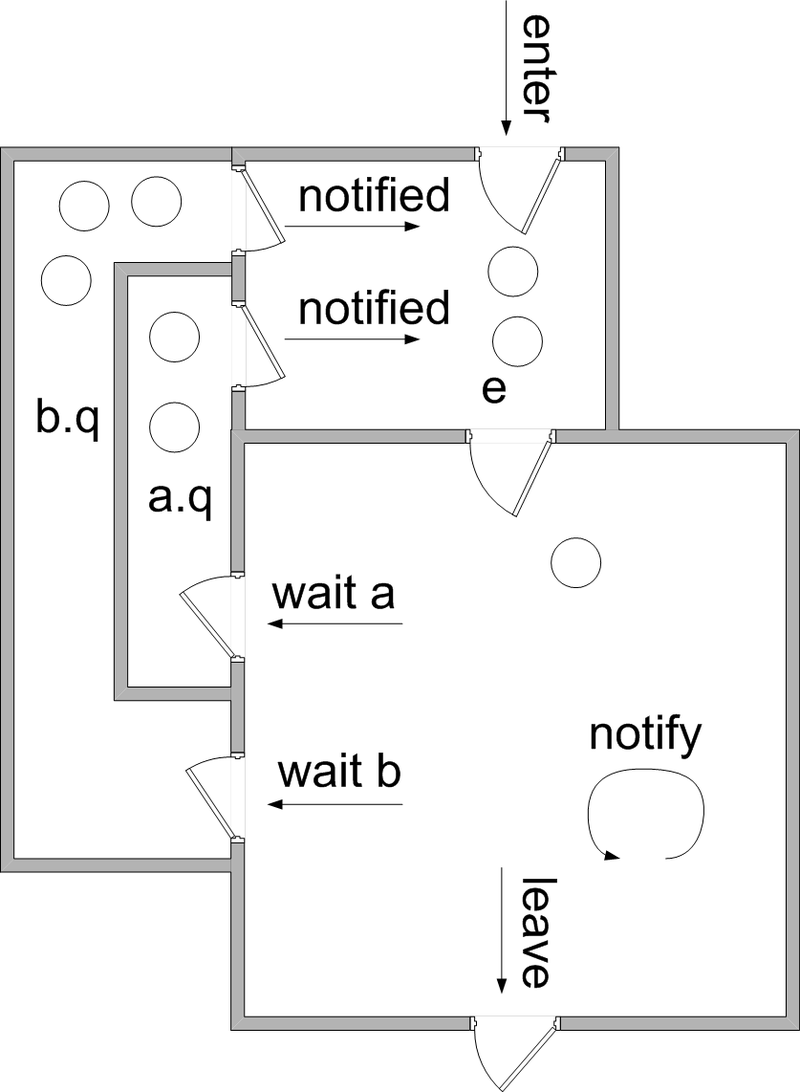
\includegraphics[width=0.35\textwidth]{./pics/CondScheme.png}};
\end{tikzpicture}

% TODO: DaveDice wait morphing pub
\end{frame}

\subsection{Concurrency hazards}
\showTOCSub

\begin{frame}[t, fragile]{Concurrency hazards}
\framesubtitle{Lost signal (race condition)}

Short description: \texttt{WaitSet} is empty due to race condition

\begin{minted}{java}
threadA() {
    lock.lock();
    try {
        ready = true; condition.signal();
    } finally { lock.unlock(); }
}
threadB() {
    lock.lock();
    try {
        condition.await()
        if (ready) doComputation();
    } finally { lock.unlock(); }
}
\end{minted}
\end{frame}


\begin{frame}[t, fragile, noframenumbering]{Concurrency hazards}
\framesubtitle{Lost signal (race condition)}

Short description: \texttt{WaitSet} is empty due to race condition

Solution: never expect that your \texttt{signal} will reach already waiting receiver. 

Sender thread:
\begin{itemize}
    \item mark ready
    \item then \texttt{signal}
\end{itemize}

Receiver thread:
\begin{itemize}
    \item check ready
    \item then \texttt{await}
\end{itemize}
\end{frame}

\questiontime{Changing two consecutive lines of code transforms program-with-bugs-in-signalling into default-concurrent-pattern. Name other concurrent primitive that has the same property.}

\begin{frame}[t,fragile]{Concurrency hazards}
\framesubtitle{Lost signal (logic error)}
Short description: \texttt{signal} delivered message to wrong waiter, \texttt{signalAll} needed

\begin{minted}[fontsize=\footnotesize]{java}
producer1() { lock.lock(); try { while (true) {
    if (data != null) condition.await();
    data = new Data1(); condition.signal();
}} finally { lock.unlock(); } 
}
producer2() { lock.lock(); try { while (true) {
    if (data != null) condition.await();
    data = new Data2(); condition.signal();
}} finally { lock.unlock(); }
}
consumer() { lock.lock(); try { while (true) {
    if (data != null) { process(data); data = null; condition.signal(); }
    condition.await();
}} finally { lock.unlock(); }
}
\end{minted}
\end{frame}


\begin{frame}[t,fragile,noframenumbering]{Concurrency hazards}
\framesubtitle{Lost signal (logic error)}
Short description: \texttt{signal} delivered message to wrong waiter, \texttt{signalAll} needed

\begin{minted}{java}
producer1() { loop-under-lock {
    if (data != null) condition.await();
    data = new Data1(); condition.signal();
}}
producer2() { loop-under-lock {
    if (data != null) condition.await();
    data = new Data2(); condition.signal();
}}
consumer() { loop-under-lock {
    if (data != null) { process(data); data = null; condition.signal(); }
    condition.await();
}}
\end{minted}
\end{frame}

\begin{frame}[t,fragile,noframenumbering]{Concurrency hazards}
\framesubtitle{Lost signal (logic error)}
Short description: \texttt{signal} delivered message to wrong waiter, \texttt{signalAll} needed

Solution:
\begin{itemize}
    \item \texttt{signalAll} is always safer, yet could be less performant. \textbf{Not always correct}.
    \item better divide responsibility across threads (one-to-one communication via personal \texttt{Condition}s? other sync primitives?)
\end{itemize}
\end{frame}

\begin{frame}[t,fragile]{Concurrency hazards}
\framesubtitle{Predicate invalidation}

Short description: thread \texttt{await}s for predicate and \textbf{does not recheck} it upon wakeup

\begin{minted}{java}
threadA() { lock.lock(); try {
        while (true) {
            if (data == null) condition.await();
            System.out.println(data.hashCode())            
        }
    } finally { lock.unlock(); } 
}
threadB() { while (true) {
        lock.lock(); try {
            if (random.nextBoolean()) { data = null; } 
            else { data = new Data(); condition.signal(); }
        } finally { lock.unlock(); }
    }
}
\end{minted}
\end{frame}

\begin{frame}[t,fragile,noframenumbering]{Concurrency hazards}
\framesubtitle{Predicate invalidation}

Short description: thread \texttt{await}s for predicate and \textbf{does not recheck} it upon wakeup

Solution: \textbf{always} re-check \texttt{await} predicate. If it is invalidated, wait again. 

\textbf{Ensure} you are not suffering from missing signal bug.
\end{frame}


\begin{frame}[fragile]{Concurrency hazards}
\framesubtitle{Spurious wakeup}

Short description: thread wake-ups for no reason\footnote{\url{https://linux.die.net/man/3/pthread_cond_wait}}\footnote{\url{https://devblogs.microsoft.com/oldnewthing/20180201-00/?p=97946}}

\begin{minted}{java}
main() {
    lock.lock();
    try {
        condition.await();
        System.out.println("Should not reach here");
    } finally { lock.unlock(); }    
}
\end{minted}

\pause

Solution:
\begin{itemize} 
    \item always wrap \texttt{await} into \texttt{while} loop with predicate re-check
    \item always expect that \texttt{await} is implemented as \texttt{unlock(); sleep(1); lock();}
\end{itemize}
\end{frame}

\questiontime{Concurrency is hard by itself! Why would library designers allow such a counter-intuitive behaviour as ''spurious wakeup''?}

\begin{frame}{Homework}

\begin{homeworkmail}{Task \taskEmpireCond}{
    Open \url{https://deadlockempire.github.io}, pass ''Condition Variables'' level.
}
\end{homeworkmail}

\end{frame}


\subsection{Performance hazards}

\begin{frame}[t,fragile]{Performance hazards}
\framesubtitle{Fairness/Starvation}

Short description: fair mutex + unfair \texttt{WaitSet} => unfair system

\begin{minted}{java}
threadA() { loop-under-lock { System.out.println("A");
                              condition.signal(); condition.await();
}}
threadB() { loop-under-lock { System.out.println("B");
                              condition.signal(); condition.await();
}}
threadC() { loop-under-lock { System.out.println("C");
                              condition.signal(); condition.await();
}}
\end{minted}

\pause
\texttt{A, B, A, B, A, B ...}

\end{frame}


\begin{frame}[t,fragile,noframenumbering]{Performance hazards}
\framesubtitle{Fairness/Starvation}

Short description: fair mutex + unfair \texttt{WaitSet} => unfair system

\
\

\texttt{WaitSet} admission policy have similar throughput/latency trade-offs as for \texttt{EnterSet}/\texttt{ArriveSet} in mutex

\
\

General note: if your algorithm have a choice ''whom to wake-up'', you have an admission policy design space
\end{frame}

\begin{frame}{Condition variable}
\framesubtitle{Conclusion}

\begin{itemize}
    \item Cross-thread message passing/coordination \textbf{could} be implemented via mutex + polling
    \item Signalling saves computation resources for something more useful than busy looping
\end{itemize}

Mutex + ConditionalVariable allow to build custom synchronization protocols. Be aware of
\begin{itemize}
    \item Lost signal problem
    \item Predicate invalidation
    \item Spurious wakeup
    \item Fairness considerations
\end{itemize}
\end{frame}

\section{Summary}

\begin{frame}{Summary}

Some data races and race conditions could be avoided by mutual exclusion.

\texttt{Mutex} (a.k.a. \texttt{lock}, a.k.a. \texttt{critical section}) provides easy-to-use and simple API.

Do not forget to keep an eye on
\begin{itemize}
    \item safety/correctness, liveness/progress guarantees, visibility/consistency, performance
\end{itemize}

Use suitable locking policies for your use-cases
\begin{itemize}
    \item code locking, data locking, lock splitting
\end{itemize}

Remember to document locking policy to keep your program modular/reusable.

Do not forget to read documentation of thread-safe classes you use.

Condition variable allows to replace polling with OS-level signalling.

Signalling protocols must be aware of
\begin{itemize}
    \item lost signals, predicate invalidation, spurious wakeups, fairness
\end{itemize}
\end{frame}

\begin{frame}{Summary: homework}

\begin{itemize}
    \item find out if asynchronous exceptions are compatible with concurrent primitives (Task~\taskAsyncException)
    \item \url{https://deadlockempire.github.io/} ''Locks'' (Task~\taskEmpire)
    \item solve Dining philosophers problem (Task~\taskCodeDining)
    \item \url{https://deadlockempire.github.io/} ''Condition Variables'' (Task~\taskEmpireCond)
\end{itemize}
\end{frame}


%Big homework (4w)
    %bounded thread pool, blocking awaits are self-helping,
%- design
%- tests
%- deadlock conditions
%- example of deadlock with resource-constrained cause


% \begin{frame}{Producer consumer}
% Unbounded queue with mutex
% \end{frame}
% 
% \begin{frame}{Publisher-subsrciber}
% Pull/push approaches, reactive systems
% \end{frame}
% 
% \begin{frame}{Backoff policies}
% Livelock
% \end{frame}
% 
% \begin{frame}{Problems}
% 
% message passing + backpressure 
% self impl thread-safe counter
% self impl striped lock (hashmap?)
% \end{frame}


\end{document}
